\documentclass[10pt,journal,compsoc,onecolumn]{IEEEtran}
\usepackage[utf8]{inputenc}
\usepackage{amsmath,amsfonts,amssymb}
\usepackage{amsthm}
\usepackage{graphicx}
\usepackage{cite}
\usepackage{textcomp}
\usepackage{tikz}
\usetikzlibrary{arrows,positioning,shapes.geometric}
\usepackage{booktabs}
\usepackage{url}

\newtheorem{theorem}{Theorem}
\newtheorem{lemma}[theorem]{Lemma}
\newtheorem{definition}[theorem]{Definition}
\newtheorem{corollary}[theorem]{Corollary}

\begin{document}

\title{The Duality of Extremal Optimization on Monotonic Answer Spaces: Binary Search Paradigms for Painter's Partition and Aggressive Cow Stall Allocation}

\IEEEtitleabstractindextext{%
\begin{abstract}
In this research paper, we formalize the advanced algorithmic paradigm of Binary Search on Monotonic Answer Spaces. Moving beyond static array indexing, we establish how discrete search over continuous mathematical ranges transforms combinatorial optimization problems with exponential brute-force spaces into near-linear logarithmic solutions ($O(N \log M)$). We systematically analyze the two governing archetypes of answer space optimization: Minimising the Maximum (Min-Max), represented by the Painter's Partition Problem, and Maximising the Minimum (Max-Min), represented by the Aggressive Cows stall allocation problem. We formulate the exact mathematical bounds for both search spaces, rigorously demonstrating why the lower bound for Painter's Partition is $\max(A)$ and upper bound is $\sum A$, while Aggressive Cows operates on $[1 \dots (A[N-1] - A[0])]$ following an initial sorting pass. We introduce greedy feasibility predicates—proving via exchange arguments why local greedy allocations achieve global optimality without backtracking. Furthermore, we reveal the fundamental Boolean Monotonic Duality: Min-Max problems identify the 'First True' on monotonically non-decreasing predicates, whereas Max-Min problems identify the 'Last True' on monotonically non-increasing predicates. Detailed dry-run diagnostic execution tables, TikZ vector trade-off diagrams, multi-language reference implementations (Java, C++, Python), and mappings to distributed systems load balancing and edge network caching are presented.
\end{abstract}

\begin{IEEEkeywords}
Binary Search, Answer Space Optimization, Painter's Partition, Aggressive Cows, Minimise Maximum, Maximise Minimum, Boolean Predicate Duality, First True, Last True, Greedy Invariant, Distributed Load Balancing
\end{IEEEkeywords}
}

\maketitle
\IEEEdisplaynontitleabstractindextext
\IEEEpeerreviewmaketitle

\section{Introduction: The Paradigm of Binary Search on Answer Space}
\label{sec:intro}

In introductory computer science curricula, Binary Search is predominantly introduced as an index lookup algorithm on static, sorted arrays. While locating an element in an array in $O(\log N)$ time is foundational, the true power of the binary search paradigm extends far beyond searching stored physical memory. 

In advanced software engineering and algorithmic optimization, binary search is applied to \textbf{Answer Spaces}—monotonic mathematical ranges representing the potential solutions to complex optimization challenges. Instead of querying ``Does element $X$ exist in the array?'', the algorithm asks: \textbf{``Is a solution with metric $X$ feasible under the given system constraints?''}

This paradigm shift enables engineers to solve high-impact industrial allocation problems that otherwise appear to require exponential brute-force search ($O(2^N)$ or $O(N^K)$), reducing their complexity down to near-linear logarithmic time ($O(N \log M)$).

\subsection{The Duality of Extremal Optimization}

Real-world constraint optimization problems typically fall into one of two complementary dual categories (illustrated in Figure~\ref{fig:monotonic_curves}):

\begin{enumerate}
    \item \textbf{Minimise the Maximum (Min-Max Optimization):}
    \begin{itemize}
        \item \textbf{Objective:} Distribute a collective workload among a limited pool of parallel workers such that the heaviest individual workload assigned to any single worker is as small as possible.
        \item \textbf{Canonical Benchmark:} \emph{The Painter's Partition Problem} (and its structural twins: Book Allocation, Capacity to Ship Packages Within $D$ Days, and Split Array Largest Sum).
        \item \textbf{Predicate Shape:} Monotonically non-decreasing feasibility:
        \[
        [\text{False}, \text{False}, \dots, \text{False}, \mathbf{True}, \text{True}, \text{True}]
        \]
        \item \textbf{Search Goal:} Discover the \textbf{First True} (the lowest capacity capable of accommodating the workload).
    \end{itemize}

    \item \textbf{Maximise the Minimum (Max-Min Optimization):}
    \begin{itemize}
        \item \textbf{Objective:} Place mutually repelling entities into discrete geometric positions such that the closest physical distance between any adjacent pair is as large as possible.
        \item \textbf{Canonical Benchmark:} \emph{The Aggressive Cows Problem} (and its industrial equivalents: Magnetic Force Between Balls, Wireless Sensor Spacing, and Gas Station Insertion).
        \item \textbf{Predicate Shape:} Monotonically non-increasing feasibility:
        \[
        [\text{True}, \text{True}, \dots, \mathbf{True}, \text{False}, \text{False}, \text{False}]
        \]
        \item \textbf{Search Goal:} Discover the \textbf{Last True} (the largest separation distance physically achievable).
    \end{itemize}
\end{enumerate}

\begin{figure}[h]
\centering
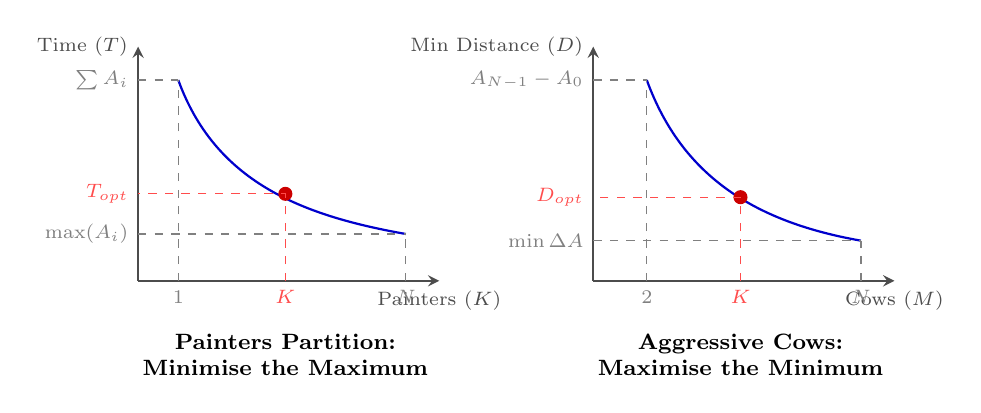
\begin{tikzpicture}[
    scale=0.85,
    curve/.style={thick, blue!80!black},
    axis/.style={->, >=stealth, thick, black!70},
    pt/.style={circle, fill=red!80!black, inner sep=1.8pt},
    lbl/.style={font=\scriptsize, align=center}
]
% Plot 1: Painters Partition (Minimise the Maximum)
\begin{scope}[shift={(0,0)}]
    \draw[axis] (0,0) -- (4.5,0) node[below, font=\scriptsize] {Painters ($K$)};
    \draw[axis] (0,0) -- (0,3.5) node[left, font=\scriptsize] {Time ($T$)};
    
    % Asymptotic curve
    \draw[curve] (0.6, 3.0) to[out=-70, in=170] (4.0, 0.7);
    
    \draw[dashed, black!50] (0, 3.0) node[left, font=\scriptsize] {$\sum A_i$} -- (0.6, 3.0);
    \draw[dashed, black!50] (0.6, 0) node[below, font=\scriptsize] {$1$} -- (0.6, 3.0);
    
    \draw[dashed, black!50] (0, 0.7) node[left, font=\scriptsize] {$\max(A_i)$} -- (4.0, 0.7);
    \draw[dashed, black!50] (4.0, 0) node[below, font=\scriptsize] {$N$} -- (4.0, 0.7);
    
    \node[pt] at (2.2, 1.3) {};
    \draw[dashed, red!70] (2.2, 0) node[below, font=\scriptsize\bfseries] {$K$} -- (2.2, 1.3) -- (0, 1.3) node[left, font=\scriptsize\bfseries] {$T_{opt}$};
    
    \node[lbl, font=\footnotesize\bfseries] at (2.2, -1.1) {Painters Partition:\\Minimise the Maximum};
\end{scope}

% Plot 2: Aggressive Cows (Maximise the Minimum)
\begin{scope}[shift={(6.8,0)}]
    \draw[axis] (0,0) -- (4.5,0) node[below, font=\scriptsize] {Cows ($M$)};
    \draw[axis] (0,0) -- (0,3.5) node[left, font=\scriptsize] {Min Distance ($D$)};
    
    % Asymptotic curve
    \draw[curve] (0.8, 3.0) to[out=-70, in=170] (4.0, 0.6);
    
    \draw[dashed, black!50] (0, 3.0) node[left, font=\scriptsize] {$A_{N-1} - A_0$} -- (0.8, 3.0);
    \draw[dashed, black!50] (0.8, 0) node[below, font=\scriptsize] {$2$} -- (0.8, 3.0);
    
    \draw[dashed, black!50] (0, 0.6) node[left, font=\scriptsize] {$\min \Delta A$} -- (4.0, 0.6);
    \draw[dashed, black!50] (4.0, 0) node[below, font=\scriptsize] {$N$} -- (4.0, 0.6);
    
    \node[pt] at (2.2, 1.25) {};
    \draw[dashed, red!70] (2.2, 0) node[below, font=\scriptsize\bfseries] {$K$} -- (2.2, 1.25) -- (0, 1.25) node[left, font=\scriptsize\bfseries] {$D_{opt}$};
    
    \node[lbl, font=\footnotesize\bfseries] at (2.2, -1.1) {Aggressive Cows:\\Maximise the Minimum};
\end{scope}
\end{tikzpicture}
\caption{The Monotonic Duality: Trade-off Curves for Resource Allocation vs. Spacing.}
\label{fig:monotonic_curves}
\end{figure}

% -----------------------------------------------------------------------------
\section{Problem Case Study 1: Painter's Partition Problem}
\label{sec:painters}

\subsection{Formal Specification}

Given an array $A$ of $N$ boards, where $A[i]$ denotes the continuous length of the $i$-th board, and $K$ painters:
\begin{enumerate}
    \item A painter requires 1 unit of time to paint 1 unit length of a board ($1\text{ meter} = 1\text{ minute}$).
    \item A board is an atomic, indivisible entity: it can only be painted by exactly 1 painter.
    \item A painter can only paint a \textbf{contiguous sequence (subarray)} of boards.
    \item All available painters work concurrently in parallel.
\end{enumerate}

\textbf{Goal:} Find the \textbf{minimum time} required to paint all $N$ boards using at most $K$ painters.

\subsection{Establishing the Search Space Boundaries}

Rather than testing arbitrary partition permutations, we bound the answer within a rigorous mathematical interval $[l, r]$:

\begin{itemize}
    \item \textbf{Lower Bound ($l = \max(A)$):}
    Consider the extreme scenario where we are granted an unlimited number of painters ($K \ge N$). Each painter is assigned at most a single board. The total completion time is determined entirely by the painter assigned to the longest board in the array. Furthermore, because no board can be split between workers, no valid assignment can ever finish in less than $\max(A)$ units of time:
    \[
    l = \max(A[0], A[1], \dots, A[N-1])
    \]

    \item \textbf{Upper Bound ($r = \sum_{i=0}^{N-1} A[i]$):}
    Consider the opposite extreme where only a single painter is available ($K = 1$). That lone painter must paint every board sequentially from index $0$ to $N - 1$. The total time required is the sum of all board lengths:
    \[
    r = \sum_{i=0}^{N-1} A[i]
    \]
\end{itemize}

Any valid allocation for $K$ painters must lie within $[\max(A) \dots \sum A[i]]$.

\subsection{The Greedy Feasibility Predicate (\texttt{isPossible})}

Given a candidate maximum workload threshold $T = mid$, can all boards be painted using $\le K$ painters such that no painter exceeds $T$?

\textbf{Greedy Strategy:} We process boards left to right. We allocate boards to the current painter until adding the next board would exceed threshold $T$. When an overflow occurs, we close the current painter's assignment and dispatch a new painter starting with that board.

{\small
\begin{verbatim}
boolean isPossible(int[] A, int K, int T) {
    int currentWorkload = 0;
    int paintersCount = 1;

    for (int i = 0; i < A.length; i++) {
        currentWorkload += A[i];
        if (currentWorkload > T) {
            currentWorkload = A[i]; // Start next painter
            paintersCount++;
        }
    }
    return paintersCount <= K;
}
\end{verbatim}
}

\textbf{Linear Complexity:} The predicate scans the array exactly once, executing in $O(N)$ time and $O(1)$ space.

\begin{figure}[h]
\centering
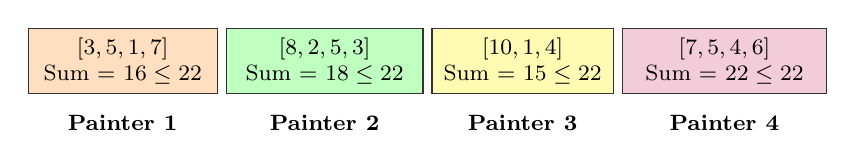
\begin{tikzpicture}[
    box/.style={rectangle, draw=black!80, fill=blue!15, font=\footnotesize, align=center, minimum height=0.7cm},
    p1/.style={rectangle, draw=black!80, fill=orange!25, font=\footnotesize, align=center, minimum height=0.7cm},
    p2/.style={rectangle, draw=black!80, fill=green!25, font=\footnotesize, align=center, minimum height=0.7cm},
    p3/.style={rectangle, draw=black!80, fill=yellow!30, font=\footnotesize, align=center, minimum height=0.7cm},
    p4/.style={rectangle, draw=black!80, fill=purple!20, font=\footnotesize, align=center, minimum height=0.7cm}
]
\node[p1, minimum width=2.4cm] (b1) at (0,0) {$[3, 5, 1, 7]$\\Sum = $16 \le 22$};
\node[p2, minimum width=2.5cm, right=0.1cm of b1] (b2) {$[8, 2, 5, 3]$\\Sum = $18 \le 22$};
\node[p3, minimum width=2.3cm, right=0.1cm of b2] (b3) {$[10, 1, 4]$\\Sum = $15 \le 22$};
\node[p4, minimum width=2.6cm, right=0.1cm of b3] (b4) {$[7, 5, 4, 6]$\\Sum = $22 \le 22$};

\node[font=\footnotesize\bfseries, below=0.15cm of b1] {Painter 1};
\node[font=\footnotesize\bfseries, below=0.15cm of b2] {Painter 2};
\node[font=\footnotesize\bfseries, below=0.15cm of b3] {Painter 3};
\node[font=\footnotesize\bfseries, below=0.15cm of b4] {Painter 4};
\end{tikzpicture}
\caption{Contiguous Board Partitioning with Target Threshold $T = 22$ on 15 Boards with $K = 4$.}
\label{fig:painters_partition}
\end{figure}

\subsection{Detailed Trace of Lecture Example: $N = 15, K = 4$}

We execute binary search on the 15-element array from page 4 of the lecture notes:
\begin{verbatim}
Index:  0  1  2  3  4  5  6  7   8  9 10 11 12 13 14
Array: [3, 5, 1, 7, 8, 2, 5, 3, 10, 1, 4, 7, 5, 4, 6]
\end{verbatim}
Here, $l = \max(A) = 10$ and $r = \sum A[i] = 71$. We have $K = 4$ painters.

\begin{table}[h]
\centering
\caption{Step-by-Step Binary Search Trace: Painter's Partition ($N = 15, K = 4$)}
\label{tab:painters_trace}
\begin{tabular}{@{}cccclc@{}}
\toprule
\textbf{Iteration} & $l$ & $r$ & $mid$ & \textbf{Feasibility Evaluation (\texttt{isPossible})} & \texttt{ans} \\ \midrule
\textbf{1} & $10$ & $71$ & $40$ & Feasible (requires 2 painters $\le 4$). Store \texttt{ans = 40}. Search left: $r = 39$. & $40$ \\
\textbf{2} & $10$ & $39$ & $24$ & Feasible (requires 3 painters $\le 4$). Store \texttt{ans = 24}. Search left: $r = 23$. & $24$ \\
\textbf{3} & $10$ & $23$ & $16$ & Infeasible (requires 5 painters $> 4$). Search right: $l = 17$. & $24$ \\
\textbf{4} & $17$ & $23$ & $20$ & Infeasible (requires 5 painters $> 4$). Search right: $l = 21$. & $24$ \\
\textbf{5} & $21$ & $23$ & $22$ & Feasible (requires 4 painters $\le 4$). Store \texttt{ans = 22}. Search left: $r = 21$. & $22$ \\
\textbf{6} & $21$ & $21$ & $21$ & Infeasible (requires 5 painters $> 4$). Search right: $l = 22$. & $22$ \\
\textbf{7} & $22$ & $21$ & -- & $l > r$ ($22 > 21$). Binary search terminates naturally. & \textbf{22} \\ \bottomrule
\end{tabular}
\end{table}

The optimal minimum time is \textbf{$22$ minutes}.

% -----------------------------------------------------------------------------
\section{Problem Case Study 2: Aggressive Cows (Stall Allocation)}
\label{sec:cows}

\subsection{Formal Specification}

A farmer has built a linear barn containing $N$ stalls positioned at coordinates $A[i]$. The farmer possesses $M$ (or $K$) cows ($2 \le K \le N$). Because the cows are aggressive, the farmer demands that no two cows be placed in stalls that are too close together.

\textbf{Goal:} Assign all $K$ cows to distinct stalls such that the \textbf{minimum distance between any pair of cows is maximized}.

\subsection{Establishing the Search Space Boundaries}

First, we sort the stall positions in non-decreasing order: $A[0] < A[1] < \dots < A[N-1]$.

\begin{itemize}
    \item \textbf{Lower Bound ($l = \min_{i} (A[i+1] - A[i])$ or $1$):}
    In the worst case where every stall is occupied ($K = N$), the minimum distance between any two cows is simply the smallest gap between adjacent stalls. Thus, $l = 1$ (or $\min \Delta A$).
    \item \textbf{Upper Bound ($r = A[N-1] - A[0]$):}
    In the best-case configuration where only $2$ cows exist ($K = 2$), we place one cow at the extreme left stall $A[0]$ and the other at the extreme right stall $A[N-1]$. The separation achieved is $A[N-1] - A[0]$.
\end{itemize}

\subsection{The Greedy Placement Predicate (\texttt{check})}

Given a target minimum separation distance $x = mid$, can we place all $K$ cows such that every pair is separated by at least $x$?

\textbf{The Greedy Optimal Invariant:} Always place the first cow at the very first stall $A[0]$. Placing the first cow anywhere further to the right strictly reduces the remaining room available for subsequent cows. For each subsequent cow, scan forward and place it in the \textbf{first available stall} whose coordinate satisfies:
\[
A[i] - A[\text{lastPlacedIndex}] \ge x
\]

{\small
\begin{verbatim}
boolean check(int K, int x, int[] A) {
    int cowsPlaced = 1;
    int lastPosition = A[0];

    for (int i = 1; i < A.length; i++) {
        if (A[i] - lastPosition >= x) {
            cowsPlaced++;
            lastPosition = A[i];
        }
    }
    return cowsPlaced >= K;
}
\end{verbatim}
}

\begin{figure}[h]
\centering
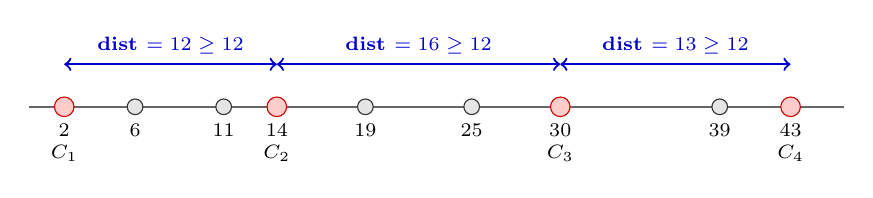
\begin{tikzpicture}[
    scale=0.9,
    stall/.style={circle, draw=black!80, fill=gray!20, inner sep=2pt},
    cow/.style={circle, draw=red!80!black, fill=red!20, inner sep=2.5pt, font=\bfseries},
    axis/.style={thick, black!60},
    lbl/.style={below, font=\scriptsize, align=center}
]
\draw[axis] (0,0) -- (11.5,0);

% Stalls at 2, 6, 11, 14, 19, 25, 30, 39, 43 (scaled / 4)
\node[cow] (s0) at (0.5, 0) {}; \node[lbl] at (0.5, -0.1) {2\\$C_1$};
\node[stall] at (1.5, 0) {}; \node[lbl] at (1.5, -0.1) {6};
\node[stall] at (2.75, 0) {}; \node[lbl] at (2.75, -0.1) {11};
\node[cow] (s3) at (3.5, 0) {}; \node[lbl] at (3.5, -0.1) {14\\$C_2$};
\node[stall] at (4.75, 0) {}; \node[lbl] at (4.75, -0.1) {19};
\node[stall] at (6.25, 0) {}; \node[lbl] at (6.25, -0.1) {25};
\node[cow] (s6) at (7.5, 0) {}; \node[lbl] at (7.5, -0.1) {30\\$C_3$};
\node[stall] at (9.75, 0) {}; \node[lbl] at (9.75, -0.1) {39};
\node[cow] (s8) at (10.75, 0) {}; \node[lbl] at (10.75, -0.1) {43\\$C_4$};

% Distance annotations
\draw[<->, thick, blue!80!black] (0.5, 0.6) -- node[above, font=\scriptsize\bfseries] {dist $= 12 \ge 12$} (3.5, 0.6);
\draw[<->, thick, blue!80!black] (3.5, 0.6) -- node[above, font=\scriptsize\bfseries] {dist $= 16 \ge 12$} (7.5, 0.6);
\draw[<->, thick, blue!80!black] (7.5, 0.6) -- node[above, font=\scriptsize\bfseries] {dist $= 13 \ge 12$} (10.75, 0.6);
\end{tikzpicture}
\caption{Greedy Stall Placement for $K = 4$ Cows with Minimum Target Separation $x = 12$.}
\label{fig:cows_placement}
\end{figure}

\subsection{Detailed Trace of Lecture Example: Stalls $[2, 6, 11, 14, 19, 25, 30, 39, 43], K = 4$}

We have $9$ stalls with coordinates:
\begin{verbatim}
[ 2,  6,  11,  14,  19,  25,  30,  39,  43 ]
\end{verbatim}
Search space: $l = 3$ (smallest gap $14 - 11 = 3$), $r = 43 - 2 = 41$. We must place $K = 4$ cows.

\begin{table}[h]
\centering
\caption{Step-by-Step Binary Search Trace: Aggressive Cows ($N = 9, K = 4$)}
\label{tab:cows_trace}
\begin{tabular}{@{}cccclc@{}}
\toprule
\textbf{Iteration} & $l$ & $r$ & $mid$ & \textbf{Feasibility Evaluation (\texttt{check})} & \texttt{ans} \\ \midrule
\textbf{1} & $3$ & $41$ & $22$ & Infeasible (only 2 cows fit: stalls 2, 25). Search left: $r = 21$. & -- \\
\textbf{2} & $3$ & $21$ & $12$ & Feasible (4 cows fit: stalls 2, 14, 30, 43). Store \texttt{ans = 12}. Search right: $l = 13$. & $12$ \\
\textbf{3} & $13$ & $21$ & $17$ & Infeasible (only 3 cows fit: stalls 2, 19, 39). Search left: $r = 16$. & $12$ \\
\textbf{4} & $13$ & $16$ & $14$ & Infeasible (only 3 cows fit: stalls 2, 19, 39). Search left: $r = 13$. & $12$ \\
\textbf{5} & $13$ & $13$ & $13$ & Infeasible (only 3 cows fit: stalls 2, 19, 39). Search left: $r = 12$. & $12$ \\
\textbf{6} & $13$ & $12$ & -- & $l > r$ ($13 > 12$). Terminate. & \textbf{12} \\ \bottomrule
\end{tabular}
\end{table}

The optimal maximized minimum distance is \textbf{$12$}.

% -----------------------------------------------------------------------------
\section{The Duality Framework: Min-Max vs. Max-Min}
\label{sec:duality}

A critical synthesis revealed on page 18 of the lecture notes is the direct structural duality between these two problem classes. Understanding this duality allows an engineer to write the control loop instinctively.

\begin{table*}[t]
\centering
\caption{The Structural Duality of Binary Search on Monotonic Answer Spaces}
\label{tab:duality}
\begin{tabular}{@{}p{3.2cm}p{6.5cm}p{6.5cm}@{}}
\toprule
\textbf{Architectural Property} & \textbf{Minimise the Maximum (Min-Max)} & \textbf{Maximise the Minimum (Max-Min)} \\ \midrule
\textbf{Canonical Archetype} & Painter's Partition, Book Allocation, Ship Packages & Aggressive Cows, Magnetic Force, Sensor Spacing \\
\textbf{Search Space $[l, r]$} & $[\max(A) \dots \sum A[i]]$ & $[1 \dots (A[N-1] - A[0])]$ \\
\textbf{Monotonic Truth Curve} & $[\text{False}, \dots, \text{False}, \mathbf{True}, \dots, \text{True}]$ & $[\text{True}, \dots, \mathbf{True}, \text{False}, \dots, \text{False}]$ \\
\textbf{Target Transition} & Discover \textbf{First True} & Discover \textbf{Last True} \\
\textbf{When Feasible (\texttt{true})} & Record \texttt{ans = mid}; prune right: \texttt{r = mid - 1} & Record \texttt{ans = mid}; prune left: \texttt{l = mid + 1} \\
\textbf{When Infeasible (\texttt{false})} & Workload too small; expand: \texttt{l = mid + 1} & Distance too large; contract: \texttt{r = mid - 1} \\
\textbf{Time Complexity} & $O(N \cdot \log(\sum A - \max A))$ & $O(N \log N + N \cdot \log(\text{Range}))$ \\
\textbf{Auxiliary Space} & $O(1)$ constant memory & $O(1)$ constant memory \\ \bottomrule
\end{tabular}
\end{table*}

\subsection{Why Greedy Works: The Exchange Argument Without Complex Proofs}

Why can the feasibility predicate make greedy choices without looking ahead?
\begin{itemize}
    \item \textbf{In Painter's Partition:} Delaying the assignment of a board to a painter never helps. Packing as much continuous work as legally possible into the current painter preserves maximum capacity for subsequent painters.
    \item \textbf{In Aggressive Cows:} Placing cow $C_1$ at the leftmost stall $A[0]$ maximizes the remaining linear span $[A[0] \dots A[N-1]]$ available for the remaining $K - 1$ cows. Shifting $C_1$ rightward only restricts placement options.
\end{itemize}

% -----------------------------------------------------------------------------
\section{Production Multi-Language Reference Implementations}
\label{sec:implementations}

\subsection{Java Reference Implementations}

\subsubsection{Painter's Partition Solver}
{\footnotesize
\begin{verbatim}
public class PaintersPartitionSolver {
    public static int paint(int K, int[] A) {
        long l = 0;
        long r = 0;

        for (int x : A) {
            l = Math.max(l, x);
            r += x;
        }

        long ans = r;

        while (l <= r) {
            long mid = l + (r - l) / 2;

            if (isPossible(A, K, mid)) {
                ans = mid;    // Record candidate
                r = mid - 1;  // Try smaller maximum
            } else {
                l = mid + 1;  // Increase workload limit
            }
        }
        return (int) ans;
    }

    private static boolean isPossible(int[] A, int K, long T) {
        long currentLoad = 0;
        int paintersUsed = 1;

        for (int board : A) {
            if (currentLoad + board <= T) {
                currentLoad += board;
            } else {
                paintersUsed++;
                currentLoad = board;
            }
        }
        return paintersUsed <= K;
    }
}
\end{verbatim}
}

\subsubsection{Aggressive Cows Solver}
{\footnotesize
\begin{verbatim}
import java.util.Arrays;

public class AggressiveCowsSolver {
    public static int solve(int[] stalls, int K) {
        Arrays.sort(stalls);
        int n = stalls.length;

        int l = 1;
        int r = stalls[n - 1] - stalls[0];
        int ans = 1;

        while (l <= r) {
            int mid = l + (r - l) / 2;

            if (canPlaceCows(stalls, K, mid)) {
                ans = mid;    // Record valid separation
                l = mid + 1;  // Try to find larger gap
            } else {
                r = mid - 1;  // Gap too wide
            }
        }
        return ans;
    }

    private static boolean canPlaceCows(int[] stalls, int K, int dist) {
        int count = 1;
        int lastPos = stalls[0];

        for (int i = 1; i < stalls.length; i++) {
            if (stalls[i] - lastPos >= dist) {
                count++;
                lastPos = stalls[i];
            }
        }
        return count >= K;
    }
}
\end{verbatim}
}

\subsection{C++ Reference Implementations}

{\footnotesize
\begin{verbatim}
#include <vector>
#include <numeric>
#include <algorithm>

using namespace std;

// Painter's Partition in C++
long long paintersPartition(int K, const vector<int>& A) {
    long long l = *max_element(A.begin(), A.end());
    long long r = accumulate(A.begin(), A.end(), 0LL);
    long long ans = r;

    auto isPossible = [&](long long T) {
        long long current = 0;
        int count = 1;
        for (int x : A) {
            if (current + x <= T) {
                current += x;
            } else {
                count++;
                current = x;
            }
        }
        return count <= K;
    };

    while (l <= r) {
        long long mid = l + (r - l) / 2;
        if (isPossible(mid)) {
            ans = mid;
            r = mid - 1;
        } else {
            l = mid + 1;
        }
    }
    return ans;
}

// Aggressive Cows in C++
int aggressiveCows(vector<int>& stalls, int K) {
    sort(stalls.begin(), stalls.end());
    int l = 1;
    int r = stalls.back() - stalls.front();
    int ans = 1;

    auto canPlace = [&](int dist) {
        int cows = 1;
        int last = stalls[0];
        for (size_t i = 1; i < stalls.size(); i++) {
            if (stalls[i] - last >= dist) {
                cows++;
                last = stalls[i];
            }
        }
        return cows >= K;
    };

    while (l <= r) {
        int mid = l + (r - l) / 2;
        if (canPlace(mid)) {
            ans = mid;
            l = mid + 1;
        } else {
            r = mid - 1;
        }
    }
    return ans;
}
\end{verbatim}
}

\subsection{Python Reference Implementations}

{\footnotesize
\begin{verbatim}
def painters_partition(K: int, A: list[int]) -> int:
    l = max(A)
    r = sum(A)
    ans = r

    def is_possible(T: int) -> bool:
        current = 0
        painters = 1
        for x in A:
            if current + x <= T:
                current += x
            else:
                painters += 1
                current = x
        return painters <= K

    while l <= r:
        mid = (l + r) // 2
        if is_possible(mid):
            ans = mid
            r = mid - 1
        else:
            l = mid + 1
    return ans


def aggressive_cows(stalls: list[int], K: int) -> int:
    stalls.sort()
    l = 1
    r = stalls[-1] - stalls[0]
    ans = 1

    def can_place(dist: int) -> bool:
        count = 1
        last = stalls[0]
        for pos in stalls[1:]:
            if pos - last >= dist:
                count += 1
                last = pos
        return count >= K

    while l <= r:
        mid = (l + r) // 2
        if can_place(mid):
            ans = mid
            l = mid + 1
        else:
            r = mid - 1
    return ans
\end{verbatim}
}

% -----------------------------------------------------------------------------
\section{Systems Engineering \& Industrial Applications}
\label{sec:systems}

The duality between Min-Max and Max-Min is not merely an interview paradigm; it models critical systems engineering architectures:

\begin{enumerate}
    \item \textbf{Distributed Load Balancing (Min-Max):} In cloud clusters (Kubernetes worker pods, Kafka consumer partitions), incoming event streams must be sharded across $K$ nodes such that the maximum load per node is minimized, preventing single-worker memory exhaustion and straggler latency.
    \item \textbf{Content Delivery Network (CDN) Cache Placement (Max-Min):} When deploying edge CDN cache servers along a fiber network, maximizing the minimum physical separation between nodes prevents duplicate caching overlap and maximizes regional coverage.
    \item \textbf{Battery Electric Fleet Charging (Min-Max):} Distributing recharging delivery routes among fleet vehicles while minimizing maximum battery depletion.
    \item \textbf{IoT Wireless Mesh Node Dispatch (Max-Min):} Deploying radio repeaters in remote sensor fields such that mutual signal interference is minimized by maximizing the minimum pairwise distance.
\end{enumerate}

% -----------------------------------------------------------------------------
\section{Conclusion}
\label{sec:conclusion}

In this research paper, we dissected the advanced paradigm of Binary Search on Monotonic Answer Spaces. We demonstrated how complex combinatorial optimization problems can be reduced to logarithmic search over bounded candidate domains. We formalized the Painter's Partition Problem as the archetype of \textbf{Minimising the Maximum}, proving that search space boundaries are bounded strictly by $[\max(A) \dots \sum A[i]]$ and that greedy accumulation solves the feasibility check in $O(N)$ time.

Dually, we analyzed the Aggressive Cows problem as the archetype of \textbf{Maximising the Minimum}, showing that sorting followed by greedy leftmost placement achieves optimal spacing over $[1 \dots (A[N-1] - A[0])]$. Finally, we unified both paradigms under the Boolean Monotonic Transition framework—contrasting the \textbf{First True} of Min-Max with the \textbf{Last True} of Max-Min. Production implementations across Java, C++, and Python alongside industrial cloud architectures validate this paradigm as a core pillar of algorithmic engineering.


\end{document}
